\documentclass[shortpres]{beamer}
\usetheme{CambridgeUS}

% Depending on build configuration, one of these packages will
% enable unicode
%\usepackage[utf8]{inputenc}
\usepackage{fontspec}


%Images
\usepackage{graphicx, svg}
\usepackage{caption}

\usepackage{animate}
\usepackage{array}
\usepackage{subfig}
\usepackage{multicol}
\usepackage{color}
\usepackage{pgfplots}
\usepackage{xmpmulti}

\usepackage{algorithm,algpseudocode}  %for algorithm environmenstacle in the bathymetry to show the effect of the soruce terms in 2D.t

\setbeamertemplate{footline}
{
	\leavevmode%
	\hbox{%
		\begin{beamercolorbox}[wd=.333333\paperwidth,ht=2.25ex,dp=1ex,center]{author in head/foot}%
			\usebeamerfont{author in head/foot}\insertshortauthor%~~\beamer@ifempty{\insertshortinstitute}{}{(\insertshortinstitute)}
		\end{beamercolorbox}%
		\begin{beamercolorbox}[wd=.333333\paperwidth,ht=2.25ex,dp=1ex,center]{title in head/foot}%
			\usebeamerfont{title in head/foot}\insertshorttitle
		\end{beamercolorbox}%
		\begin{beamercolorbox}[wd=.333333\paperwidth,ht=2.25ex,dp=1ex,right]{date in head/foot}%
			\usebeamerfont{date in head/foot}\insertshortdate{}\hspace*{2em}
			\insertframenumber{} / \inserttotalframenumber\hspace*{2ex}
	\end{beamercolorbox}}%
	\vskip0pt%
}\part{title}
\beamertemplatenavigationsymbolsempty


%color specification---------------------------------------------------------------
\definecolor{TUMblue}{rgb}{0.00, 0.40, 0.74}
\definecolor{TUMgray}{rgb}{0.85, 0.85, 0.86}
\definecolor{TUMpantone285C}{rgb}{0.00, 0.45, 0.81}
\definecolor{lightblue}{rgb}{0.7529,0.8118,0.9333}

\setbeamercolor{block title}{fg=white, bg=TUMpantone285C}
\setbeamercolor{block body}{bg=lightblue}
\setbeamertemplate{blocks}[rounded][shadow=true]
%----------------------------------------------------------------------------------

\setbeamercolor{frametitle}{fg=TUMblue, bg=white}
\setbeamercolor{palette primary}{fg=TUMblue,bg=TUMgray}
\setbeamercolor{palette secondary}{use=palette primary,fg=TUMblue,bg=white}
\setbeamercolor{palette tertiary}{use=palette primary,fg=white, bg=TUMblue}
\setbeamercolor{palette quaternary}{use=palette primary,fg=white,bg=TUMpantone285C}


\setbeamercolor{title}{bg=white,fg=TUMblue}
\setbeamercolor{item projected}{use=item,fg=black,bg = lightblue}
\setbeamercolor{block title}{fg=black, bg=lightblue}
\setbeamercolor{block body}{bg=white}
\setbeamertemplate{blocks}[rounded][shadow=true]
%----------------------------------------------------------------------------------



%############### Self defined commands ##############################
\newcommand{\imgvoffset}{-20pt}
\newcommand{\texthoffset}{20pt}
\newcommand{\imgfullscale}{0.75}
\newcommand{\imgcolscale}{0.9}

\captionsetup[subfigure]{labelformat=empty}		%Disable enumeration of subfigures
%####################################################################

\usepackage{anyfontsize}

\title[{Tsunami simulation}]{Assignment 3}

\author[Bellamy, Honal, Wieser]{Gruppe 03\\George Bellamy, Christoph Honal, Felix Wieser\\\vspace{10pt}{\small Bachelorpraktikum}}

\institute[TU M\"unchen]{Technical University of Munich}

\date{5. December 2017}

\begin{document}
\maketitle

\begin{frame}{Overview}
	\begin{figure}
		\subfloat[HPC]{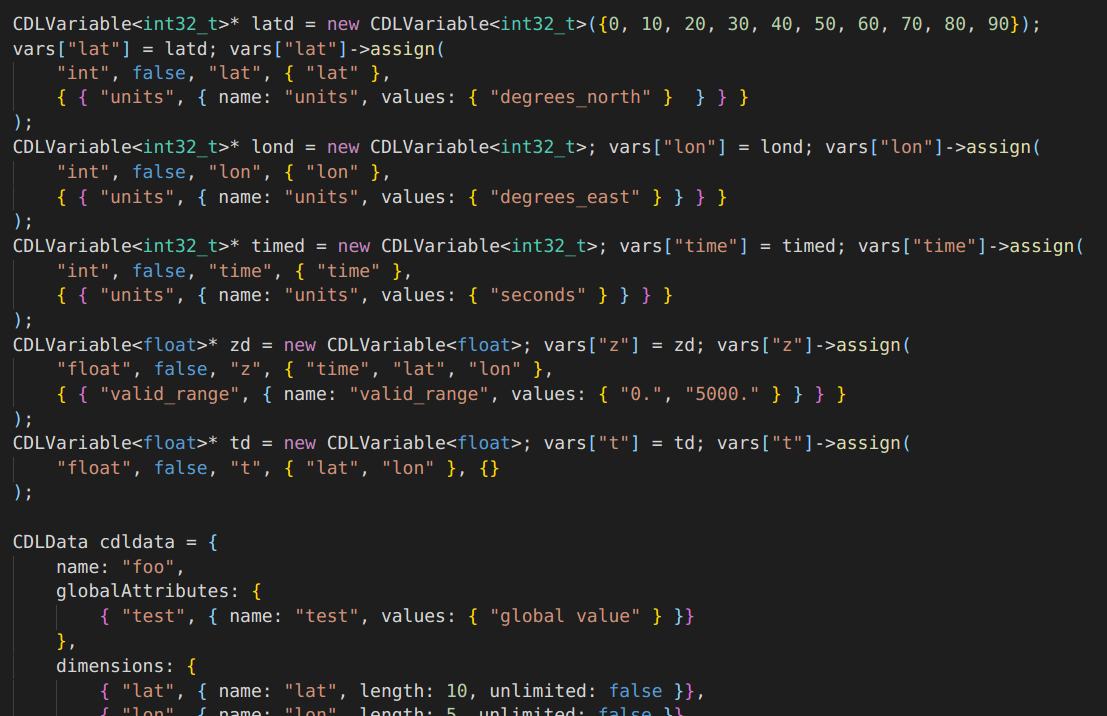
\includegraphics[clip,width=0.3\linewidth]
			{img/CDLcode.jpg}}
		\hspace{40pt}
		\subfloat[Performance analysis]{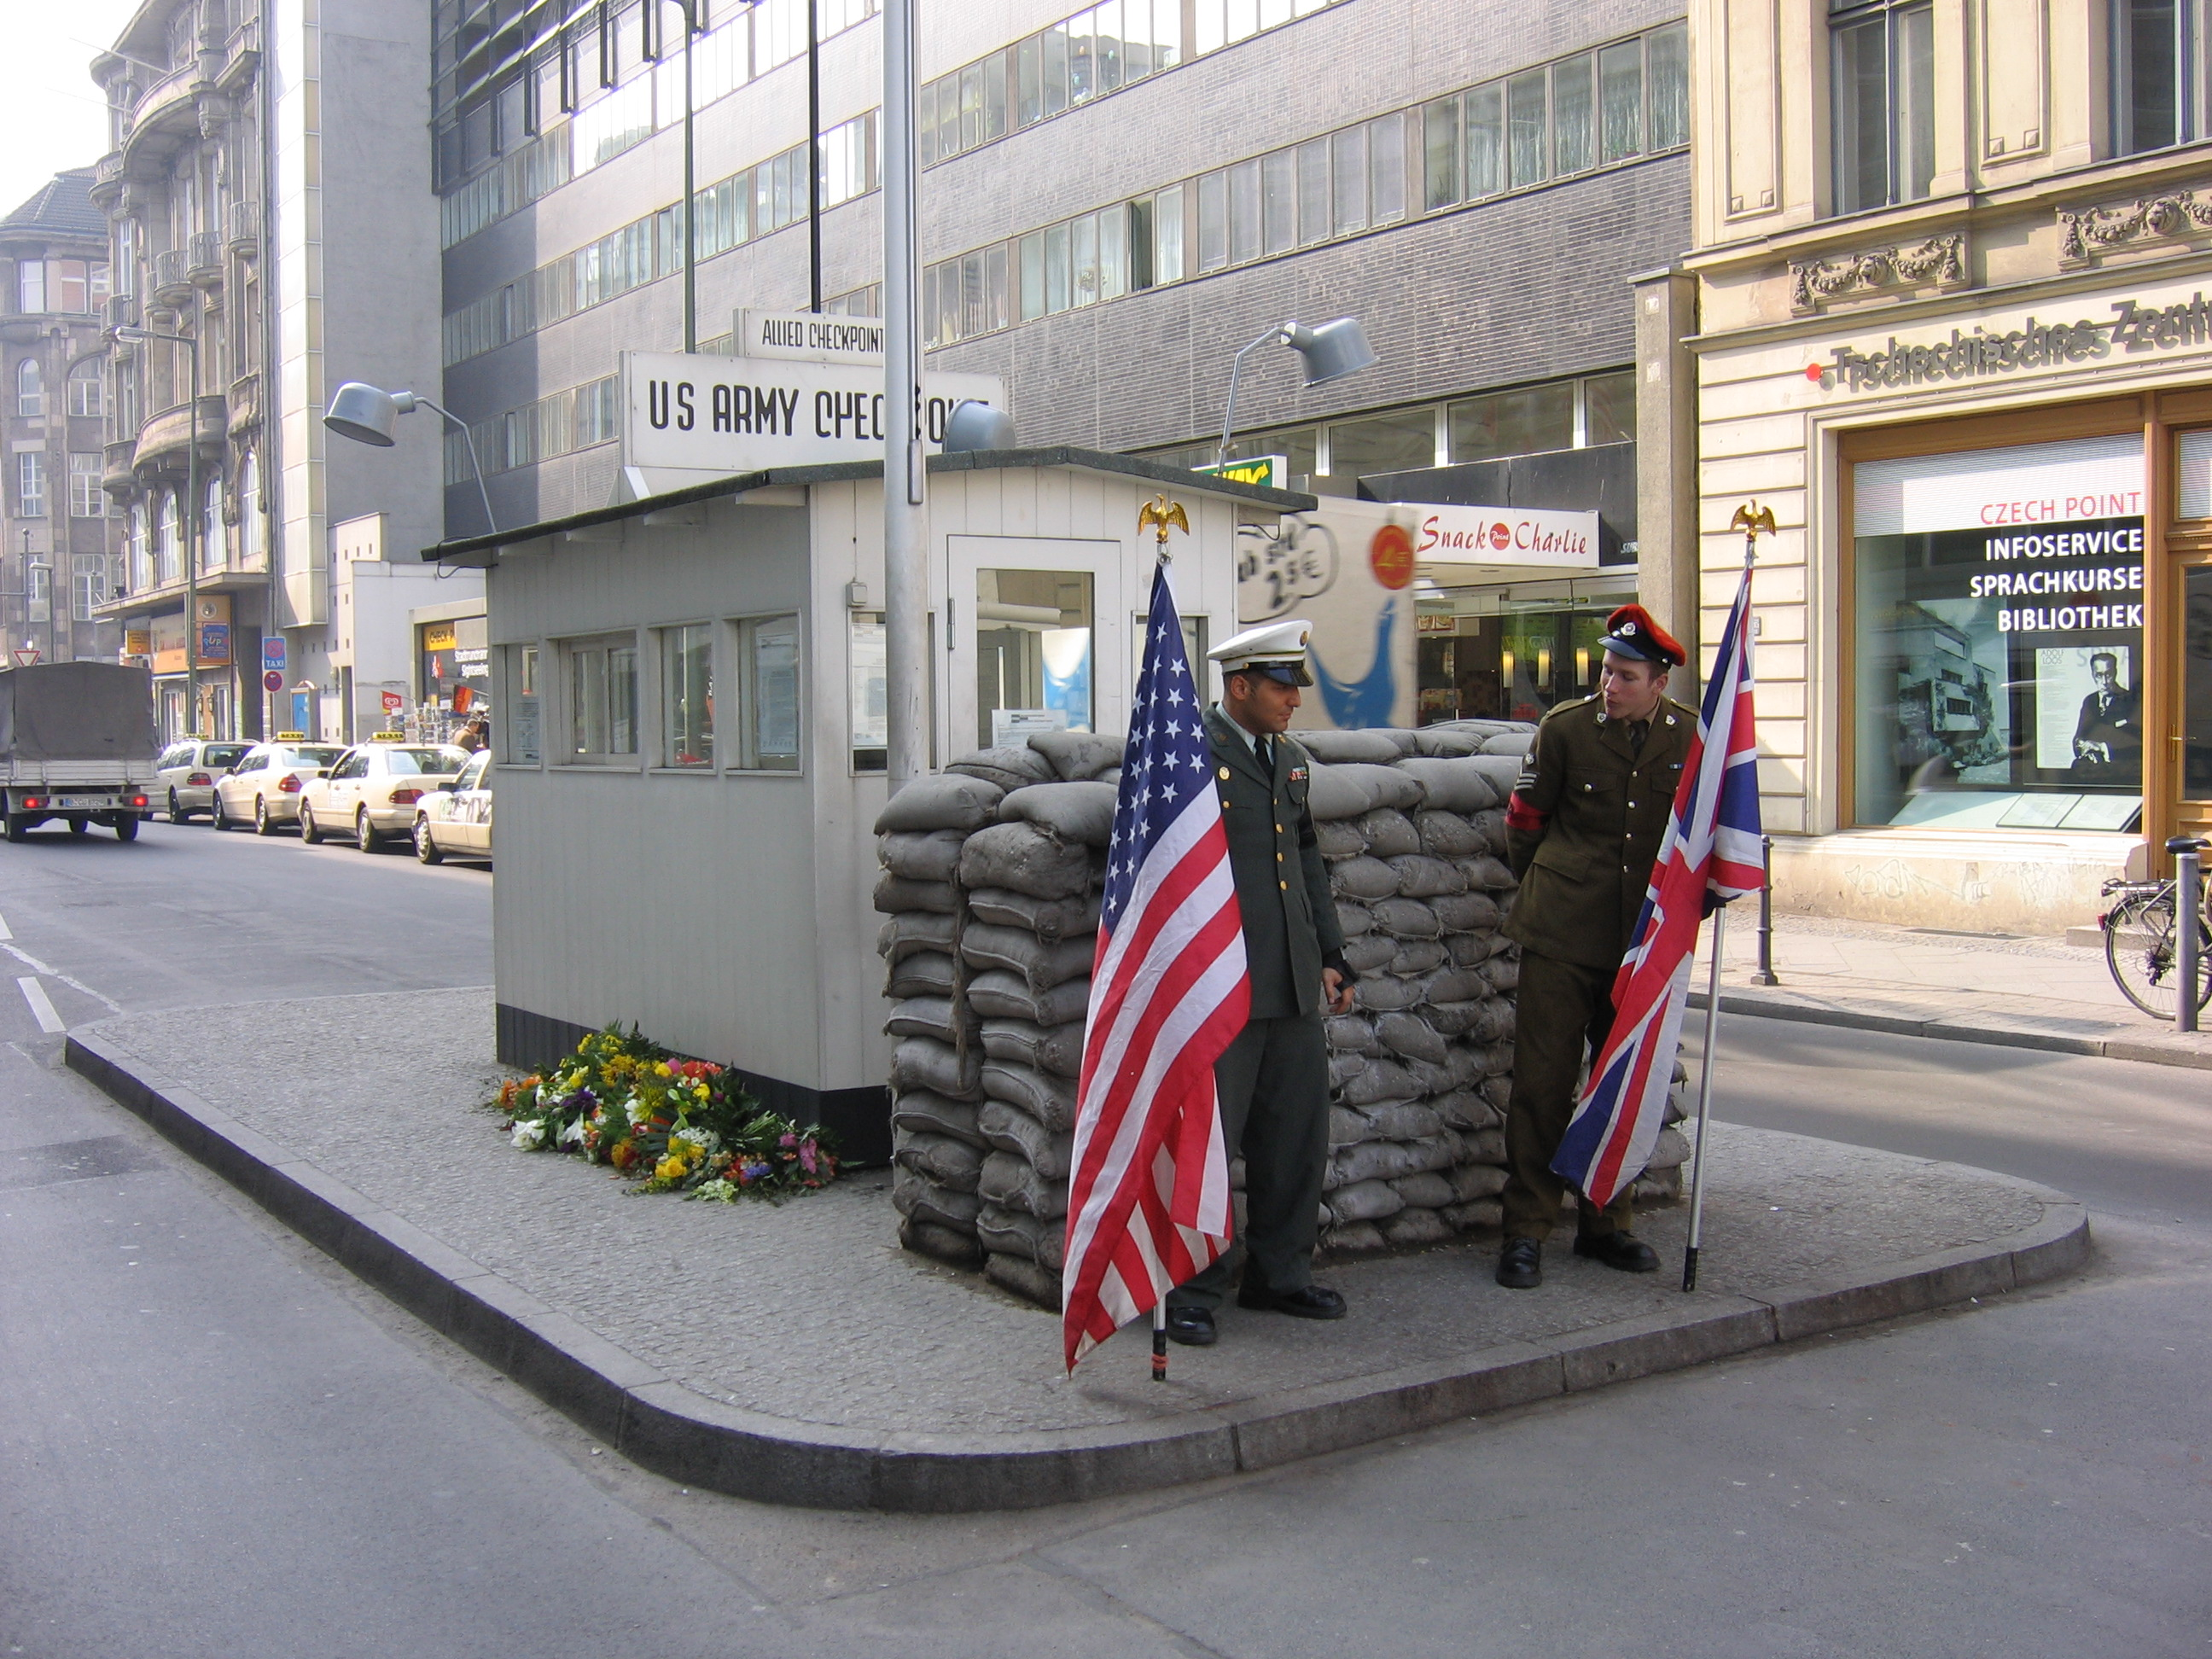
\includegraphics[clip,width=0.3\linewidth, trim={0 55pt 0 55pt}]
			{img/checkpointcharlie.jpeg}}
		\hspace{0pt}\vspace{20pt}\\
		\subfloat[OpenMP]{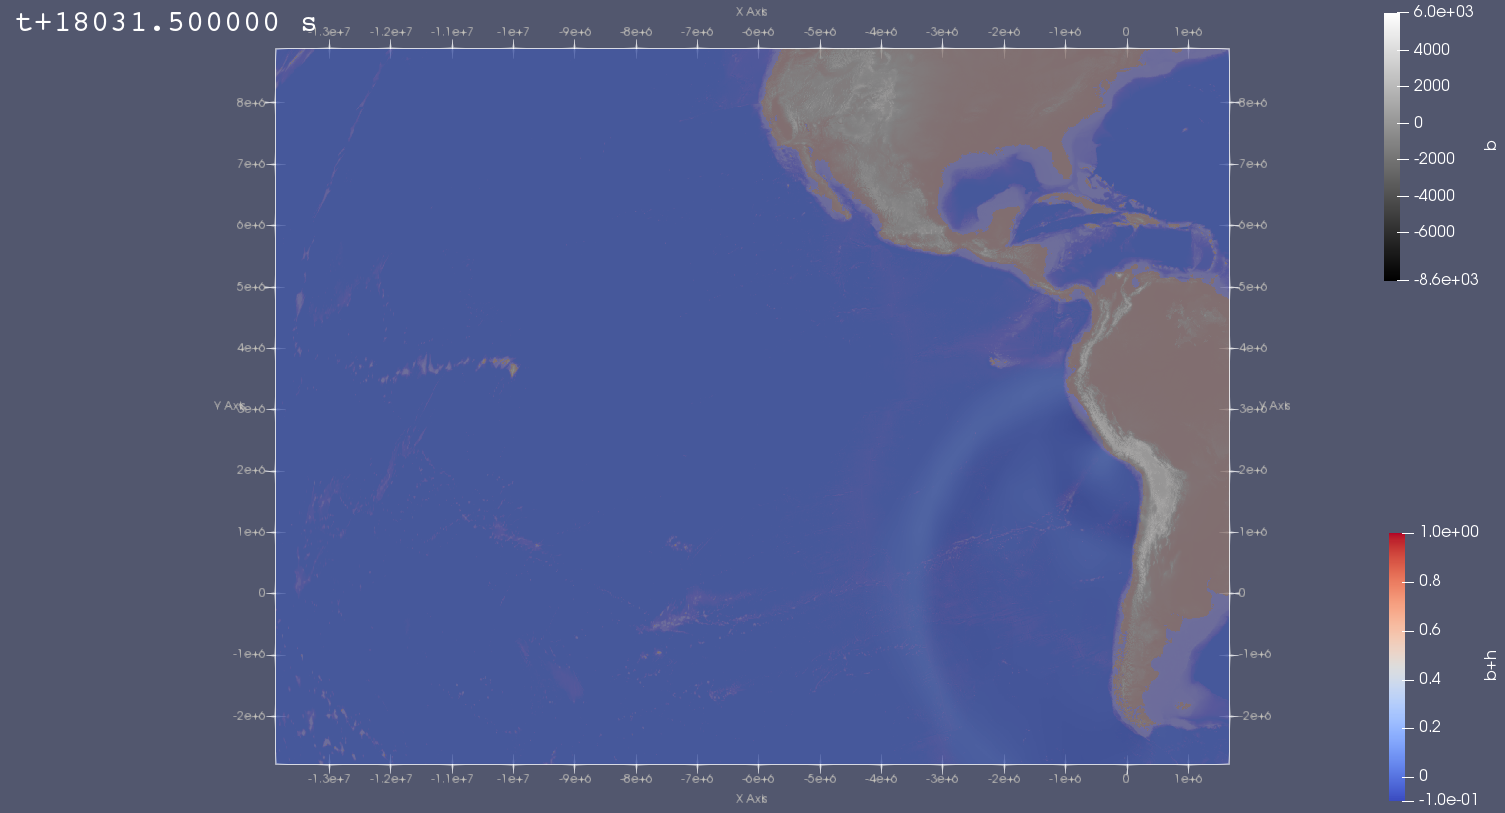
\includegraphics[clip,width=0.3\linewidth]
			{img/chile_middle_600.png}}
		\subfloat[Coarse computation]{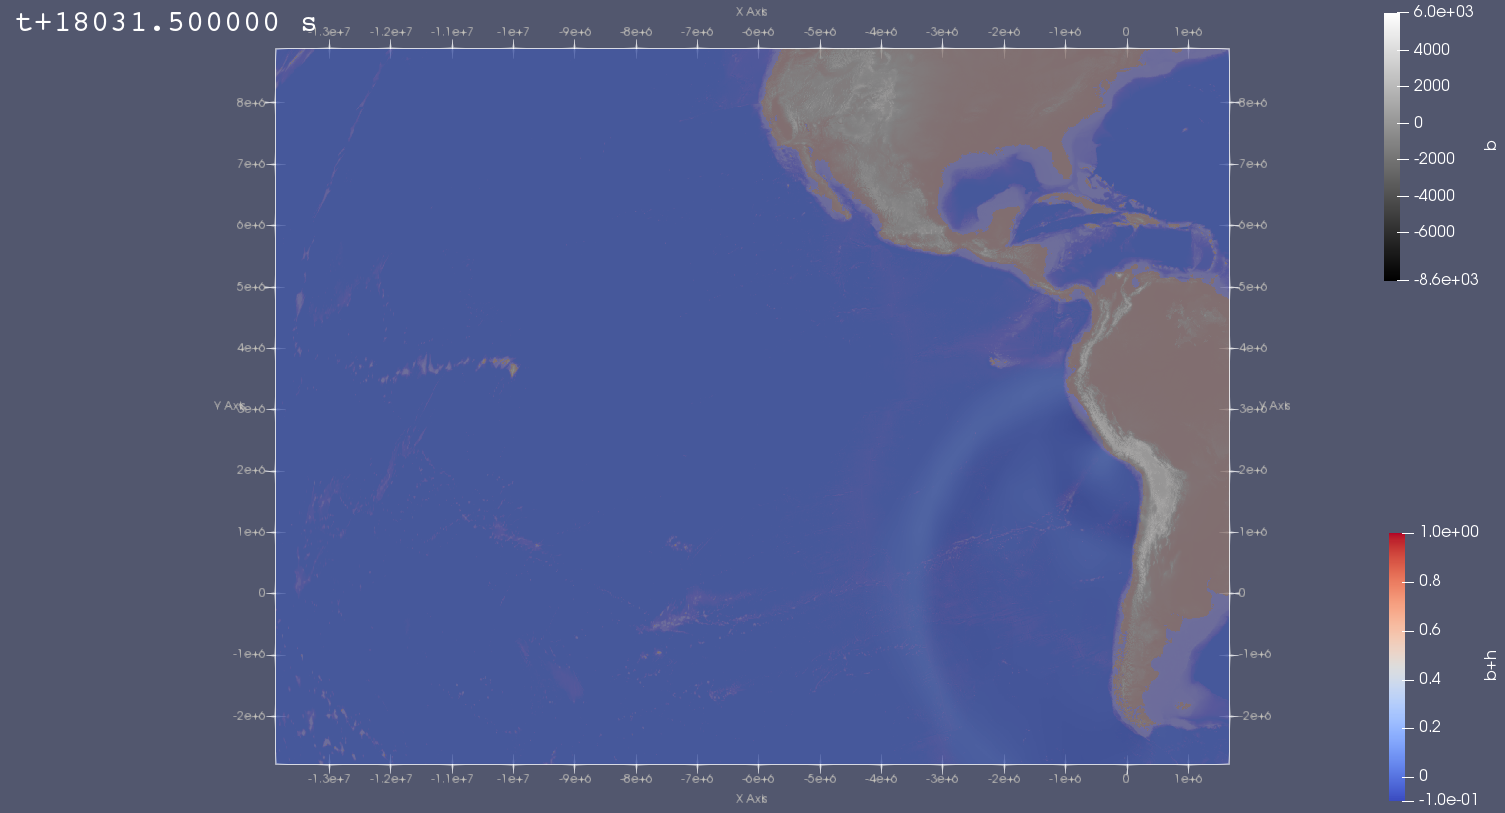
\includegraphics[clip,width=0.3\linewidth]
			{img/chile_middle_600.png}}
	\end{figure}
\end{frame}

\begin{frame}{Implementation: File parsing}
	Implementation of file reader
	\begin{itemize}
		\item \textit{NetCDFDataReader} can read bathymetry and displacement files
		\item \textit{NetCDFReader} supports meta data
	\end{itemize}
	\vspace{20pt}
	Implementation of file writer
	\begin{itemize}
		\item Flag: Append to or create new file
	\end{itemize}
\end{frame}

\begin{frame}{Implementation: Checkpointing}	
	\begin{figure}
		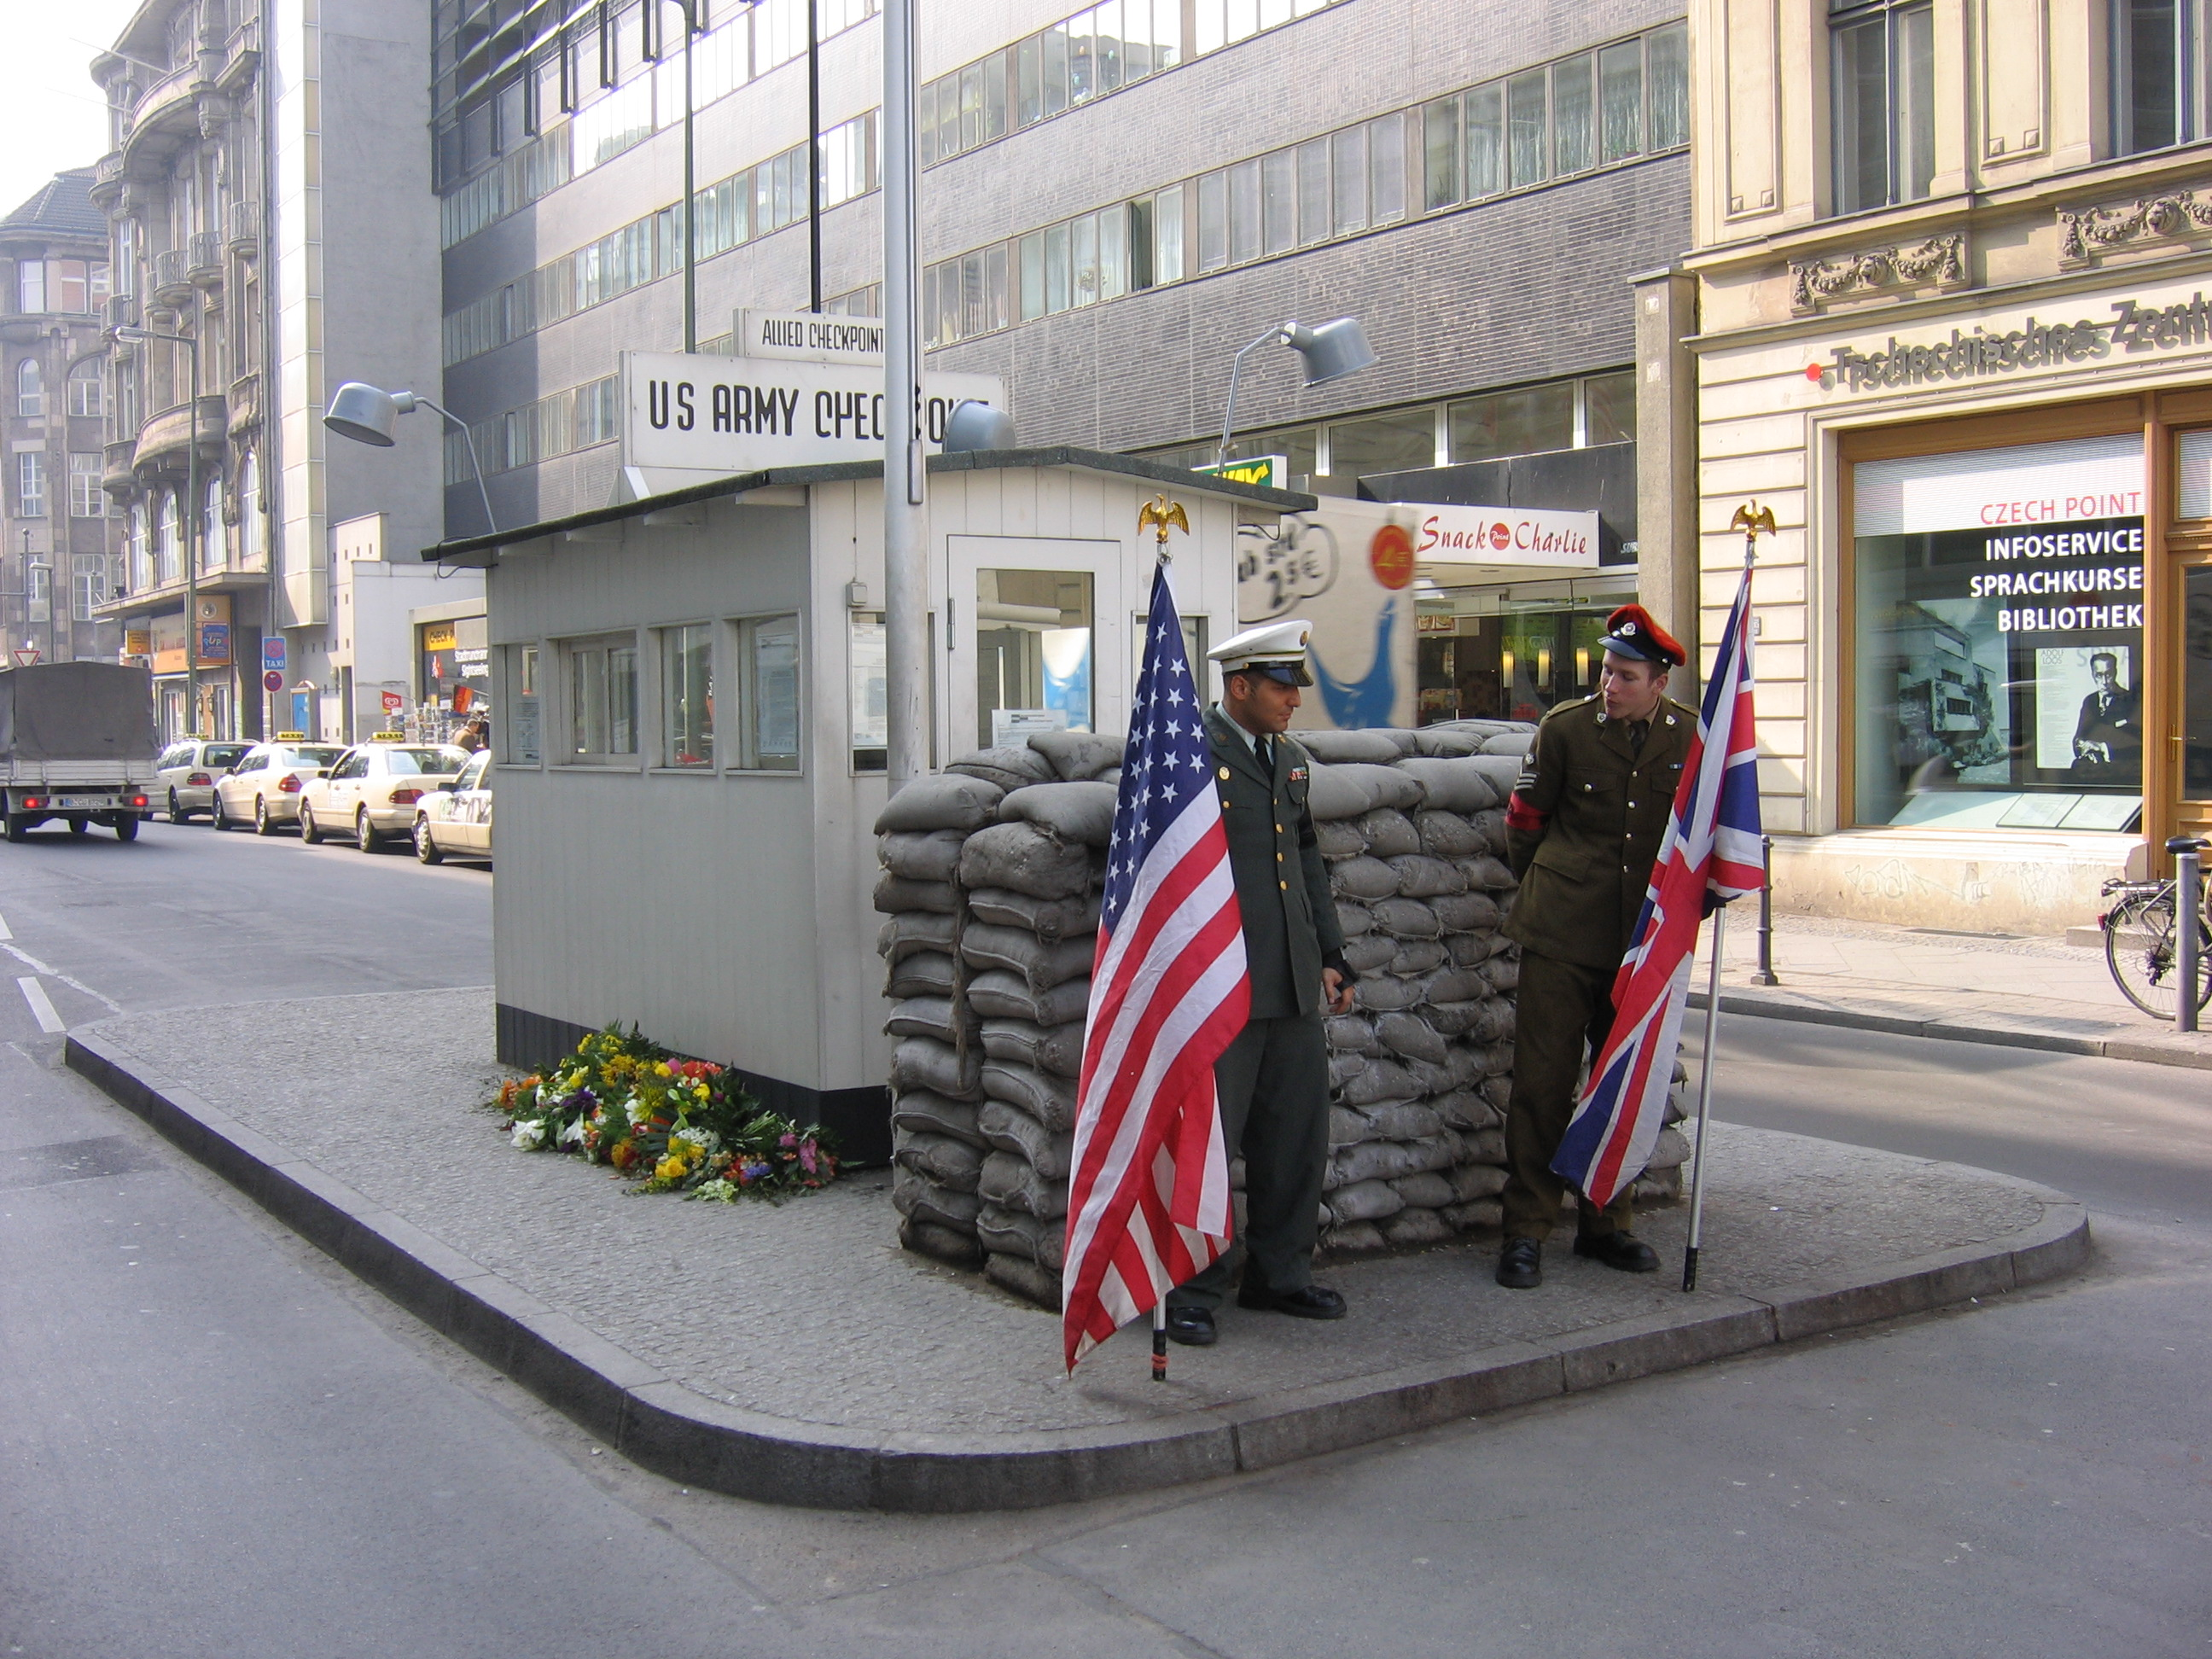
\includegraphics[width=0.3\linewidth]{img/checkpointcharlie.jpeg}
	\end{figure}
	
	\begin{itemize}
		\item Implemented netCDF-Parser for debugging purposes
		\item Enhanced \textit{NetCDFWriter} wo save meta data
		\item Implemented \textit{NetCDFDataReader}
		\begin{itemize}
			\item Customizable via command line options
			\item Can simulate crash of the application
		\end{itemize}
	\end{itemize}
	
	%------ Footer -------
	\vfill
	\flushleft
	{\fontsize{3.5}{3.5} \selectfont 
	https://s14-eu5.ixquick.com/cgi-bin/serveimage?url=https:\%2F\%2Fupload.wikimedia.org\%2Fwikipedia\%2Fcommons\%2Ff\%2Ffd\%2FCheckpoint\_Charlie\_2005\_072.JPG\&sp=2e324a64264464092e90a3097598e060}
\end{frame}

\begin{frame}{Simulation: Scenario Tohoku (2010)}
	\begin{figure}
		\only<1>{
			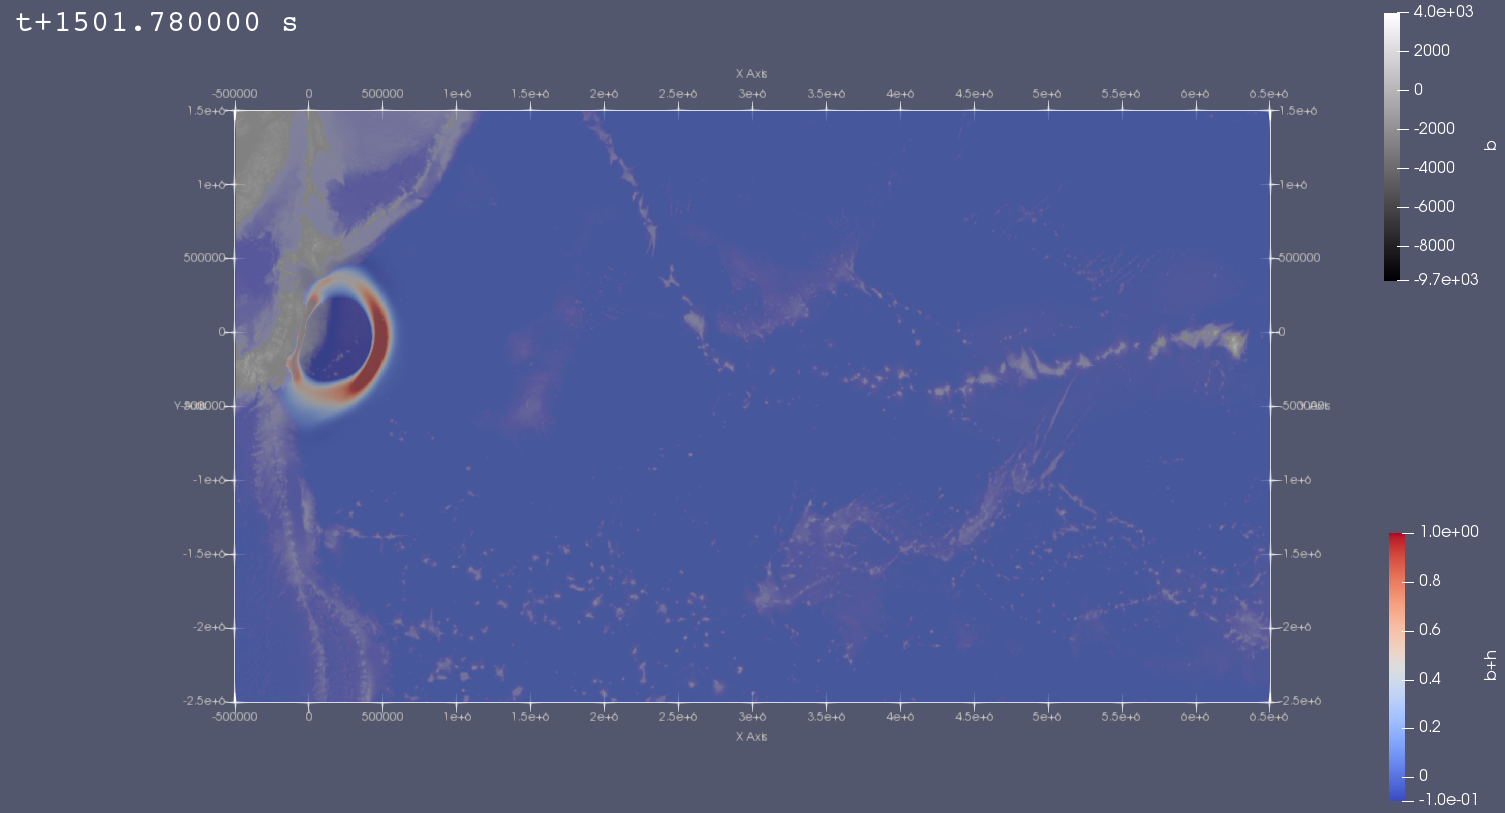
\includegraphics[width=\imgfullscale\linewidth]{img/tohoku_middle_50.png}
		}
		\only<2>{
			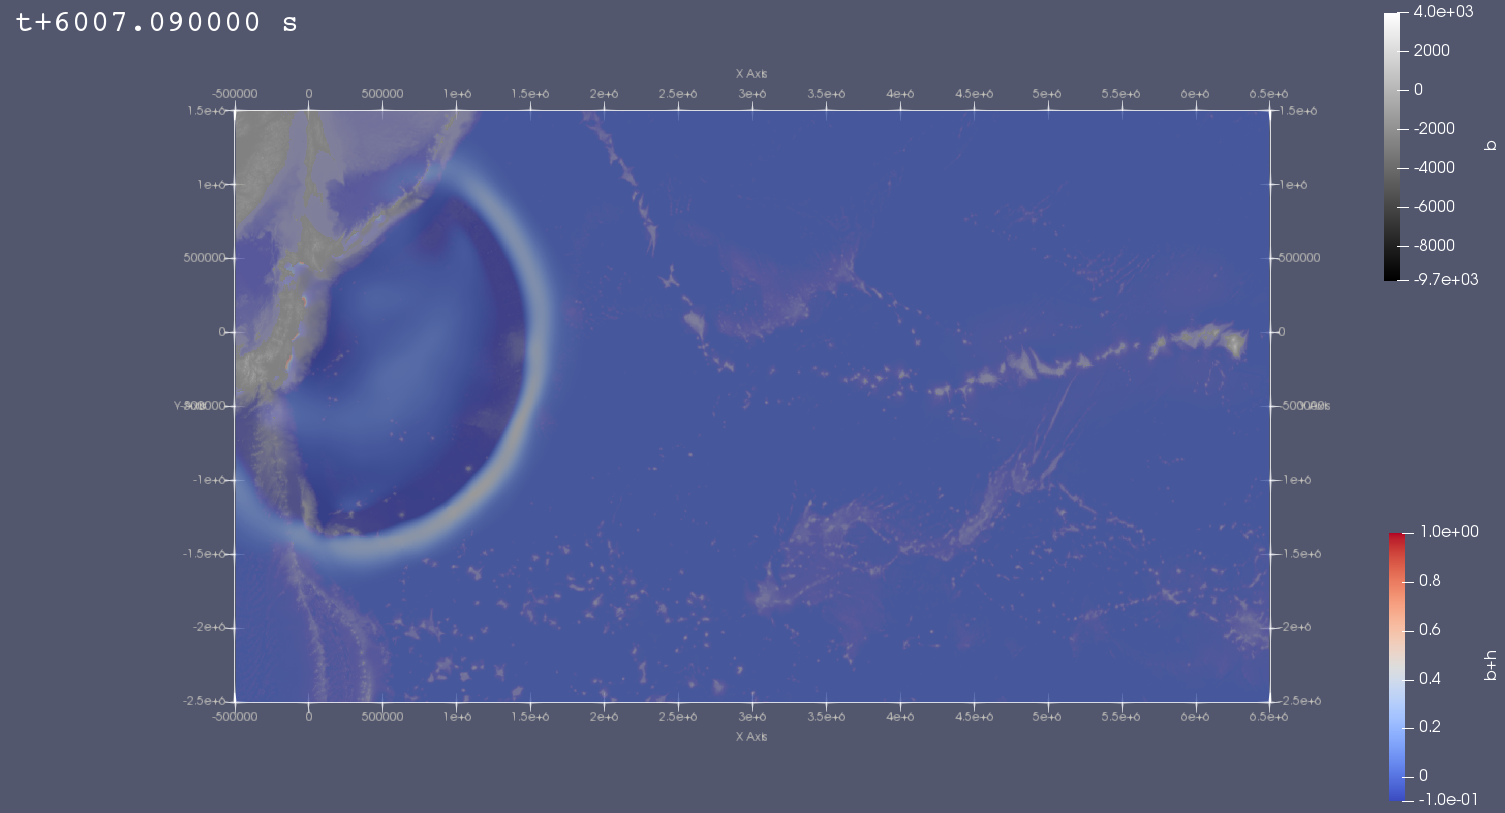
\includegraphics[width=\imgfullscale\linewidth]{img/tohoku_middle_200.png}
		}
		\only<3>{
			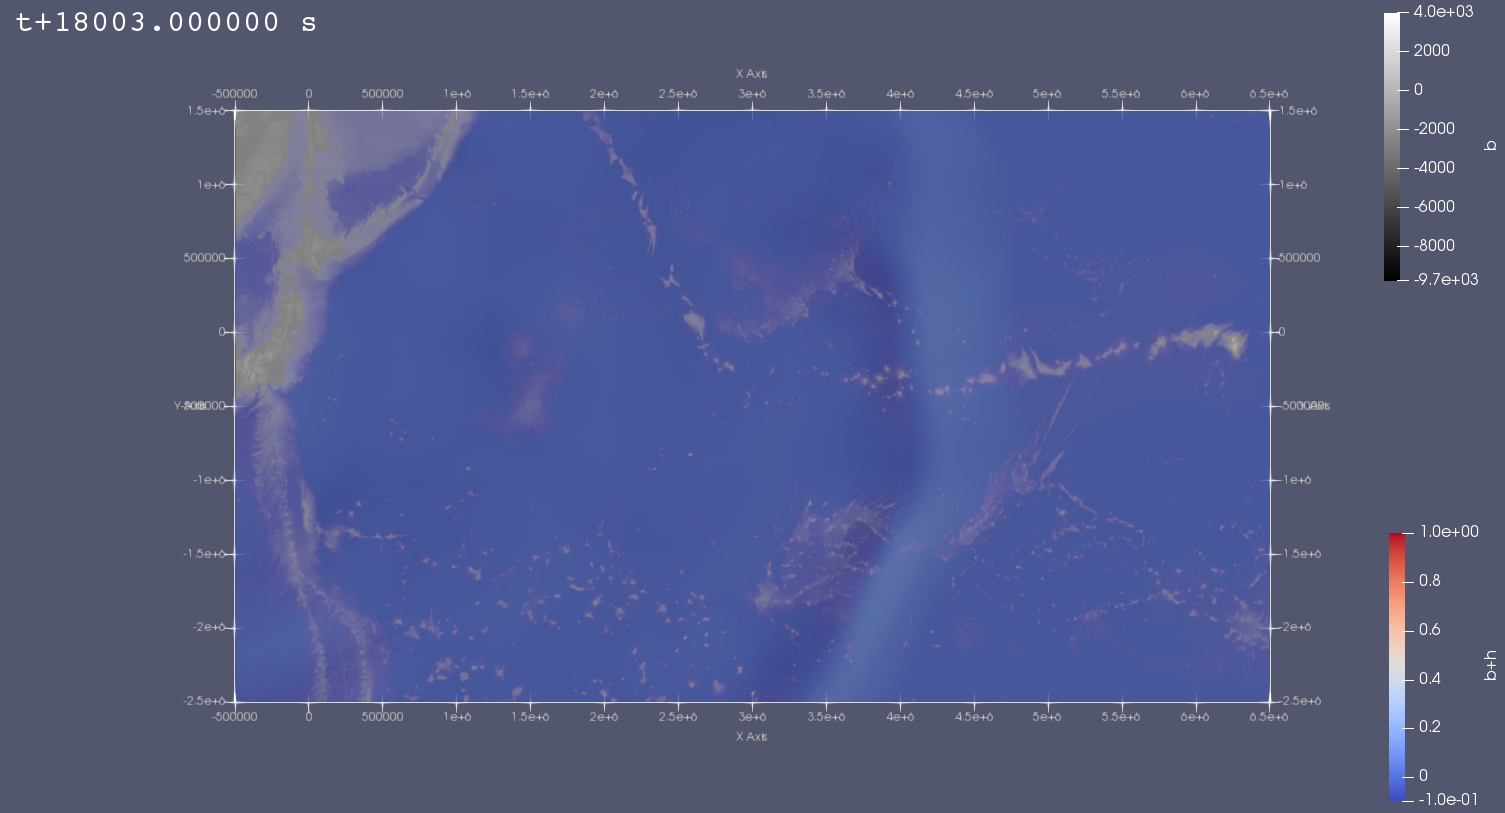
\includegraphics[width=\imgfullscale\linewidth]{img/tohoku_middle_600.png}
		}
		\caption*{Simulation visualisation}
	\end{figure}
\end{frame}

\begin{frame}{Simulation: Scenario Tohoku (2010)}
		\begin{itemize}
			\item $v \approx \sqrt{gh}$ estimates arrival after $16$ minutes
			\item UNESCO reports arrival time after $14$ minutes (maximum amplitude)
			\item Simulation calculates arrival after $14$ minutes
			\item $1000 \times 1000$ cells, each $7 km \times 4 km$
			\item $x: [-499 km; 6499 km]$ \hspace{10pt} $y: [-2499 km; 1499 km]$
			\item Wave leaves the domain as follows
		\end{itemize}
		\begin{tabular}{lll}
			North & $\approx 8500$ sec & $\approx$ $2:22$ h\\
			East & $\approx 27000$ sec & $\approx$ $7:30$ h\\
			South & $\approx 11000$ seconds & $\approx$ $3:03$ h\\
			West & $\approx 5500$ seconds & $\approx$ $1:32$ h\\
		\end{tabular}
		\vfill
		\flushleft
		{\fontsize{5}{5} \selectfont Data from: http://itic.ioc-unesco.org/images/docs/japan\_jma\_11mar11\_tsuobservations.pdf}	
\end{frame}

\begin{frame}{Simulation: Scenario Chile (2011)}
	\begin{figure}
		\centering
		\only<1>{
			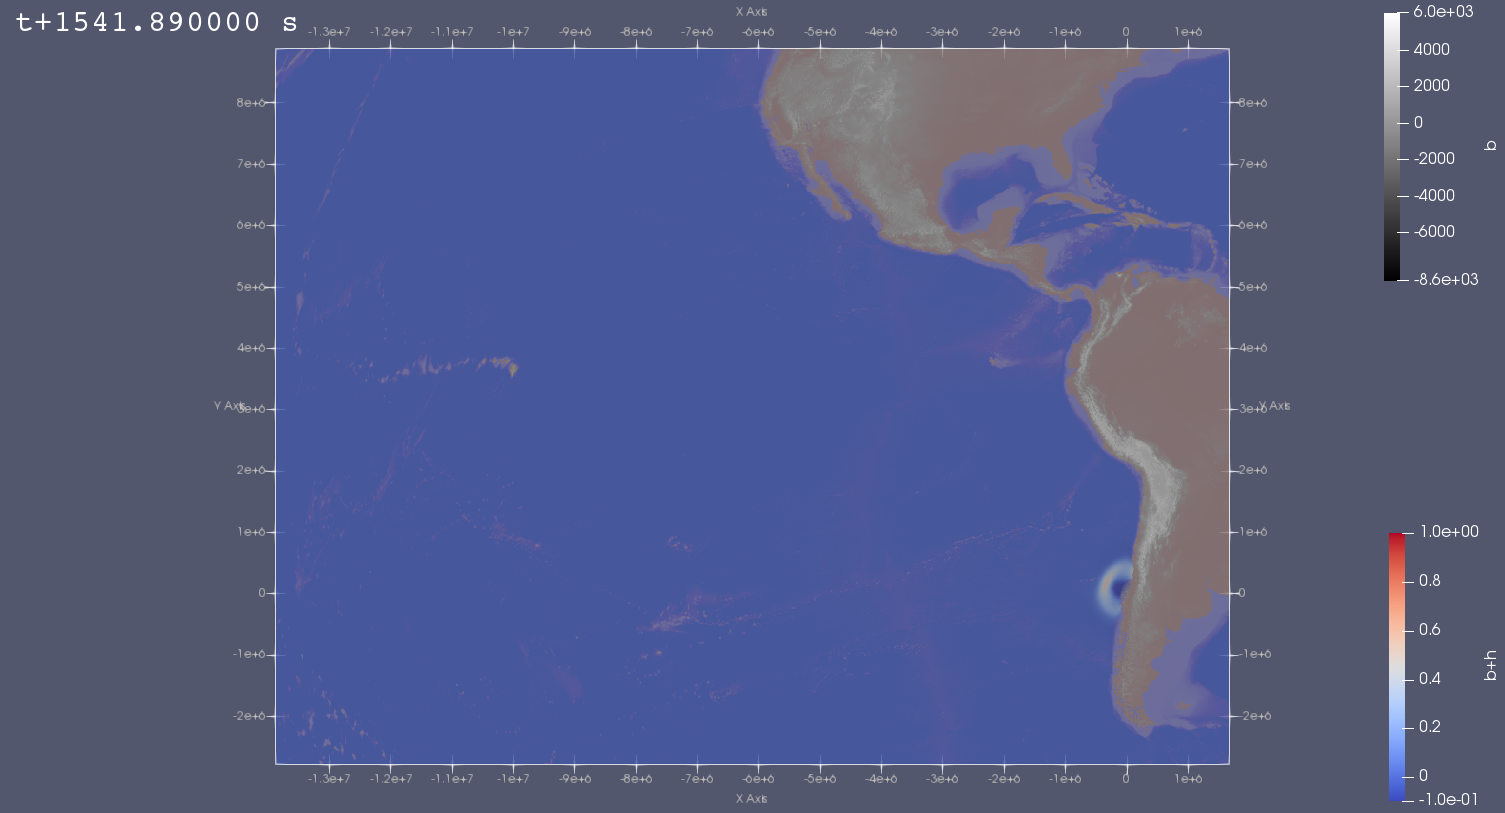
\includegraphics[width=\imgfullscale\linewidth]{img/chile_middle_50.png}
		}
		\only<2>{
			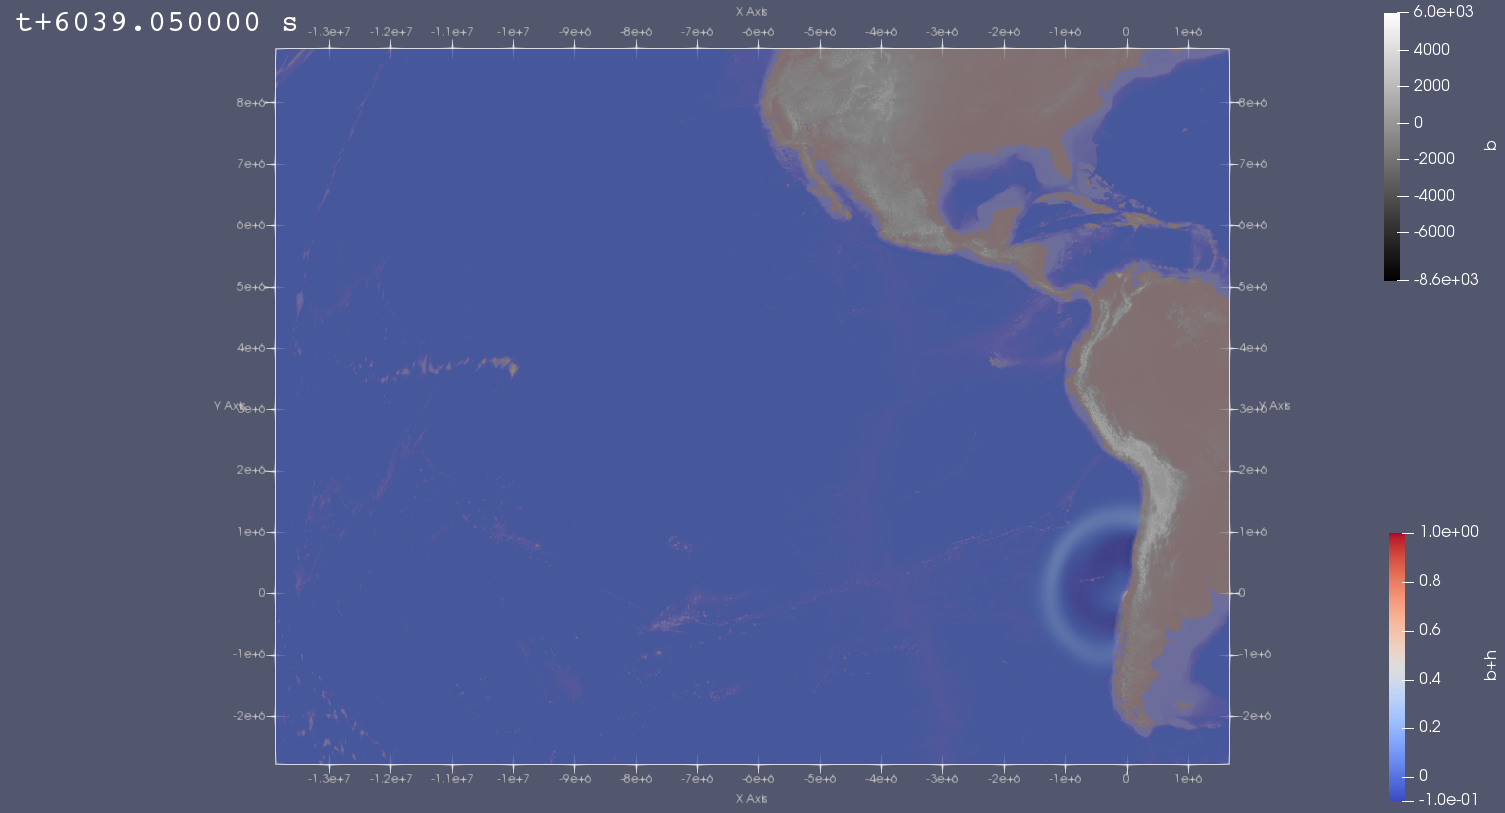
\includegraphics[width=\imgfullscale\linewidth]{img/chile_middle_200.png}
		}
		\only<3>{
			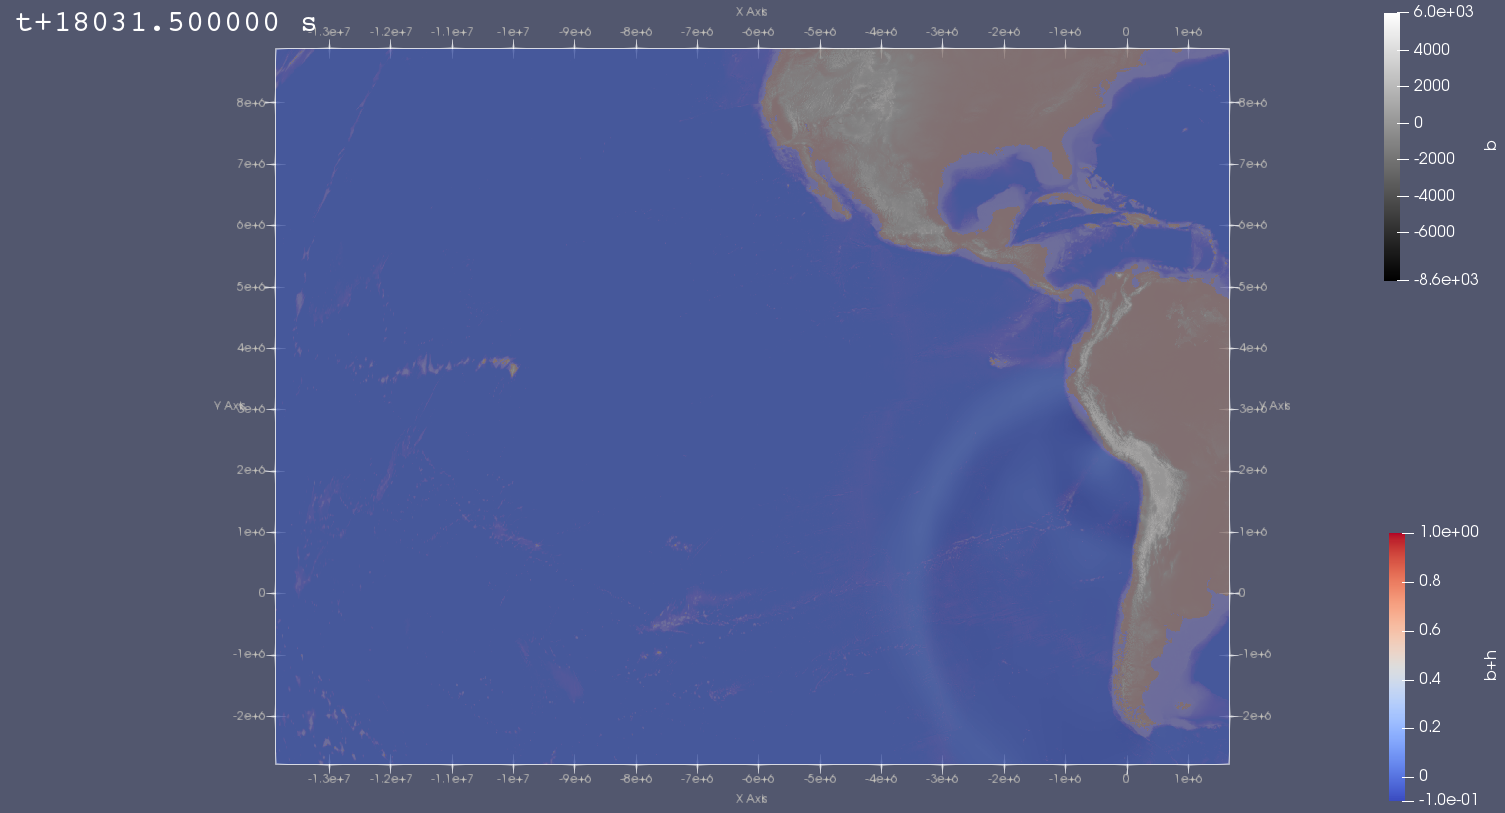
\includegraphics[width=\imgfullscale\linewidth]{img/chile_middle_600.png}
		}
		\caption*{Simulation visualisation}
	\end{figure}
\end{frame}

\begin{frame}{Simulation: Scenario Chile (2011)}
	%TODO:Add content
	\begin{figure}
		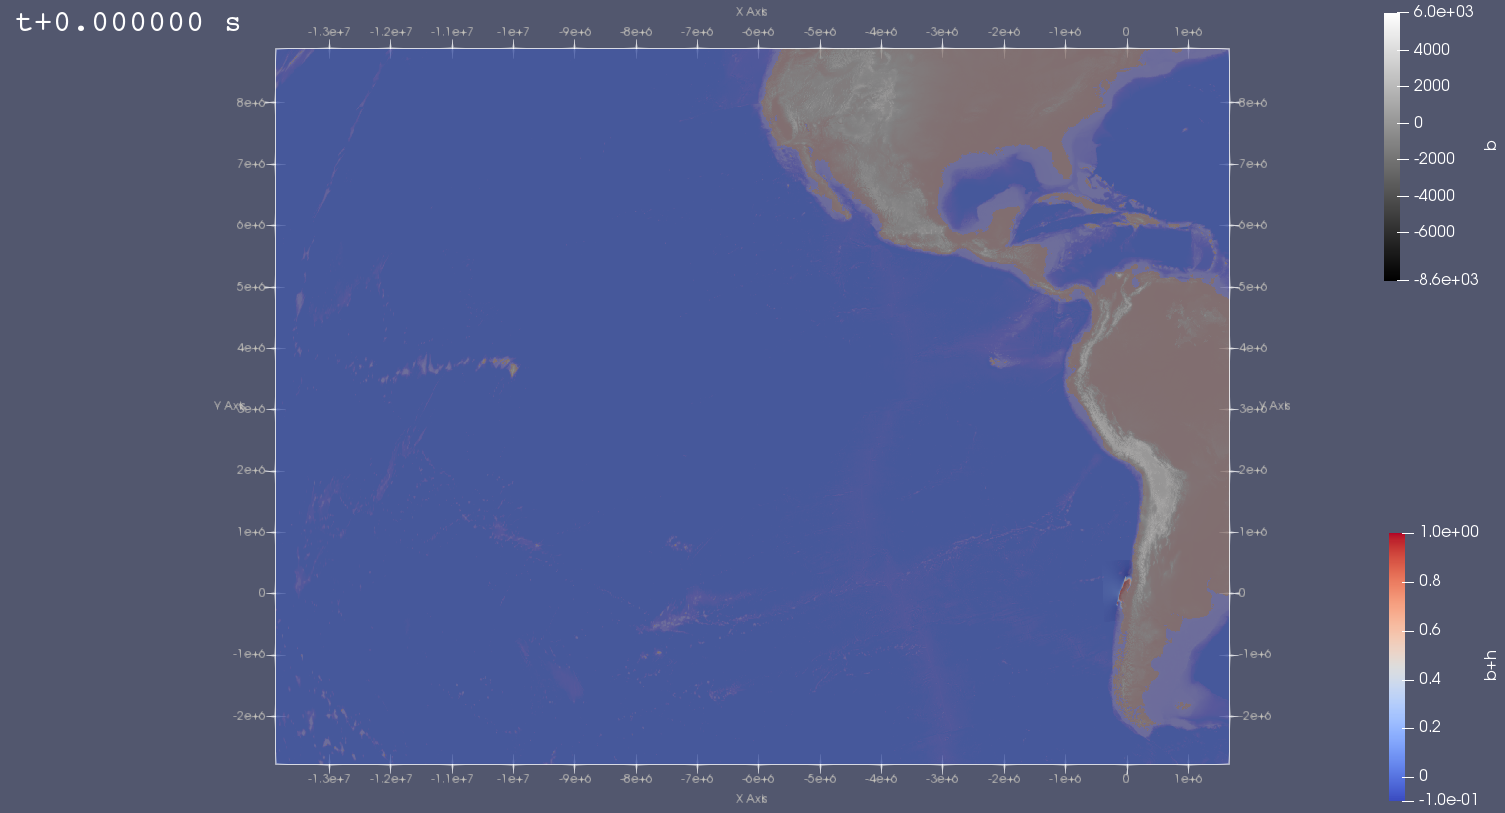
\includegraphics[width=0.6\linewidth]{img/chile_initial.png}
	\end{figure}
	\begin{itemize}
		\item Leaves the domain in the south at $\approx 4:35$ hours and dissipates before reaching the west boundary
		\item $1000 \times 1000$ cells, each $15 km \times 11.5 km$
		\item $x: [-13847 km; 1664 km]$ \hspace{10pt} $y: [-2774 km; 8879 km]$
	\end{itemize}
\end{frame}	
	
\begin{frame}{}
	\begin{figure}
		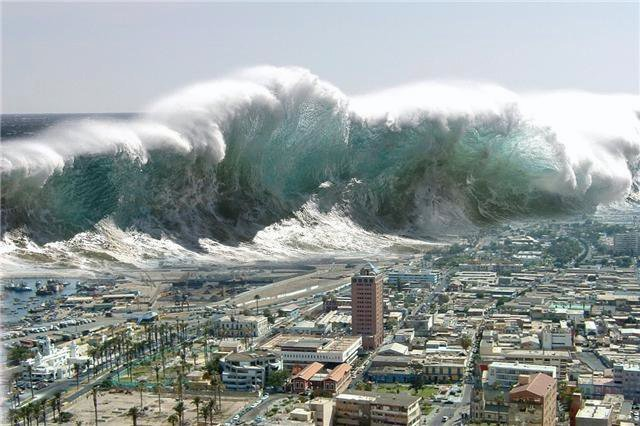
\includegraphics[clip, width=\imgfullscale\linewidth]{img/tsunami.jpg}
	\end{figure}
	\centering
	Thank you for your attention
	\\
	\vfill
	\flushleft
	{\fontsize{5}{5} \selectfont http://userscontent2.emaze.com/images/88c09d66-4283-49c0-9f80-9eb8fd05e30f/16101782-ea98-4b06-b114-4637be705926.jpg}
\end{frame}
\end{document}